\chapter{Proposed Architecture}\label{architecture}

The first $\Delta\Sigma$ modulator were first introduced by Inose, Yasuda and Murakami in 1962 \cite{first_delta}. Since then many modifications to the architecture have been proposed to improve its performance. There are four main aspects of the architecture where one can modify it: time-domain, order of the integrator, topology and the number of bits of the quantizer. In this chapter we will review the different alternatives for an architecture with respect to the four aspects. To ease the discussion, we will mainly focus on single-loop architectures since the specification given in chapter 1 only require 16 bit resolution. By designing a more complex system, we will only end up with an over-engineered proposal. 

A small discussion of the proposed architecture found in the feasibility study will be presented in the last section. The bases for the discussion is based on the well known book; \textit{Understanding Delta-Sigma Data Converters}\cite{Richard}. 

\section{Order of loop filter}

The expression of maximum SQNR for first order $\Delta\Sigma$ modulator \ref{no_noise_sqnr}, showed that for every doubling of the OSR yielded in increasing the SQNR with 9dB or ENOB with 1.5bits/octave. To be able to achieve a higher resolution (i.e., the ENOB), a larger OSR has to be used. The drawback with using a large OSR is that the correlation between the input signal and the quantization noise becomes stronger, causing correlation between white noise and idle tones which are presence inside the signal band. This causes the linear model expressed in Eq.\ref{no_noise_sqnr} to become invalid.

An obvious way to increase ENOB of the $\Delta\Sigma$ modulator is to use a high-order integrator. It can done by replacing the $\Delta\Sigma$ modulator in figure \ref{fig:linear} with \textit{L} number of $\Delta\Sigma$ modulators consecutively, where \textit{L} corresponds to the order of the integrator. The NTF can then be given by

\begin{equation}
    NTF = (1-z^{-1})^L
\end{equation}

In figures \ref{fig:SQNR} and \ref{fig:ENOB} it is shown how much OSR one need to achieve ideal SQNR and ENOB respectively, for different order of integrator. It can be observed to achieve 16 bit resolution modulators on the order of 2 and 3 is sufficient. It can also be observed that the modulator with order 2 needs much larger OSR, which can cause problems with the linear model as mentioned before.

\begin{figure}
\begin{minipage}[c]{0.5\linewidth}
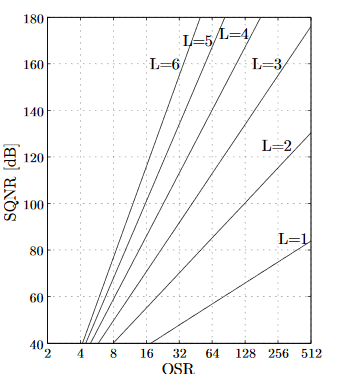
\includegraphics[width=\linewidth]{images/OSR_vs_SQNR.png}
\caption{Ideal SQNR vs OSR\cite{SQNR}}
\label{fig:SQNR}
\end{minipage}
\hfill
\begin{minipage}[c]{0.5\linewidth}%
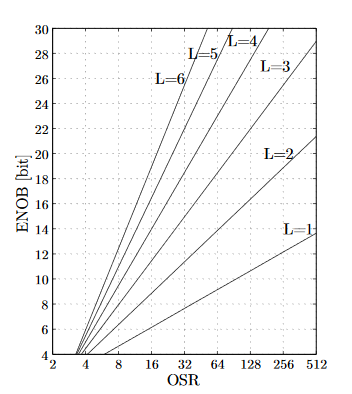
\includegraphics[width=\linewidth]{images/ENOB_vs_SQNR.png}
\caption{Ideal ENOB vs OSR\cite{SQNR}}
\label{fig:ENOB}
\end{minipage}%
\end{figure}

Instability is an issue higher-order filters are struggling with. For first and second order filters, this is not a problem, but as the order of the filters gets bigger, the out-of-band gain(OBG) of the modulator gets more aggressive. The high OBG can cause overloading of the quantizer which can make the modulator unstable. 

One can achieve stable operation by letting the input level be less or equal to the fullscale of the first feedback DAC. For high-order single-bit $\Delta\Sigma$ modulators this input range should be a few dB below the DAC fullscale\cite[Chapter 4.2]{Richard}. A rule of thumb to check if a high-order single bit $\Delta\Sigma$ modulator is stable is to use Lee's Criterion\cite{Lee}:

\begin{equation}
    |NTF_{max}| \leq 1.5
\end{equation}

where $|NTF_{max}|$ is the maximum magnitude over all frequency. Even when the criteria is fulfilled, there is a change the system will become unstable, because of the quantizer in the loop can turn the system into non-linear one\cite{Richard}. 

\section{Topologies}
The alternatives to implement a $\Delta\Sigma$ modulators can be categorized into two categories: a single-loop or a cascade architecture. The first one refer to the use of only one quantizer, as seen in the section \ref{first_order}. The other one refer to multi-stage noise-shaping (MASH) modulator which is a popular structure that eases the stability problems associated with high-order modulators. Even though it has its advantages, we will not look into MASH modulators. The single-loop architectures are simpler to design and they are able to achieve the specifications given in chapter 1 at a $\Delta\Sigma$ order of 2 and 3. We will now look at the two most used single-loop architectures; feedforward and feedback topologies. 

\subsection{Feedback topology}
The figure \ref{fig:back} depict an example of $3^{rd}$ order feedback topology. The STF and NTF for this topology is given by
\begin{equation}
    STF = \frac{b_1c_1c_2c_3H^3(z)}{1 + a_3c_3H(z) + a_2c_2c_3H^2(z) + a_1c_1c_2c_3H^3(z)}
\end{equation}

and
\begin{equation}
    NTF = \frac{1}{1 + a_3c_3H(z) + a_2c_2c_3H^2(z) + a_1c_1c_2c_3H^3(z)}
\end{equation}

Here the forward coefficients ($c_1, c_2$ and $c_3$) represent the scaling or weighed of the integrators. The purpose of them is to scale the output dynamic range of the integrators. The coefficients on the feedback path ($a_2$ and $a_3$) are used to create a transfer function that gives a stable performance, while the feedback coefficient $a_1$ ensure that the output from the quantizer tracks the input.

One of the major drawbacks with this topology is that the output swings of the integrators tends to get big, which
means that the the op-amp requirement has to be increased to avoid overloading. Furthermore the forward coefficients $c_i$ has to become smaller in order to scale down the swing. The drawback on having small coefficients is that the area to maintain the same capacitor noise gets bigger, which leads to more power to charge capacitor. Another drawback is that unlike the feedforward-path, the output of the first integrator contains some amount of the input amplitude. This leads to higher swing capabilities, which again leads to a more power-consuming system.   

\begin{figure}[H]
\centering
\begin{subfigure}[b]{0.85\textwidth}
   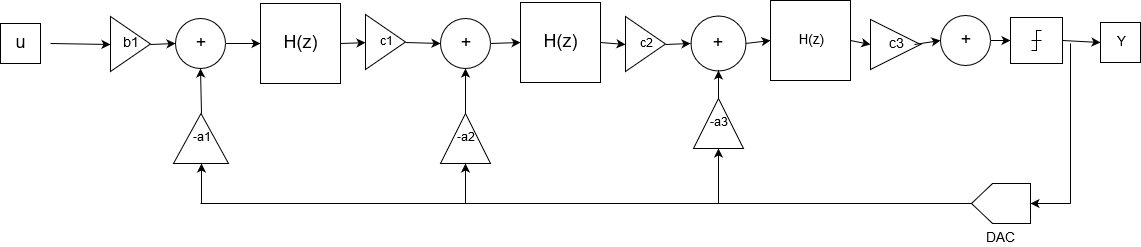
\includegraphics[width=\textwidth]{images/feedback.png}
   \caption{Feedback}
   \label{fig:back} 
\end{subfigure}

\begin{subfigure}[b]{0.85\textwidth}
   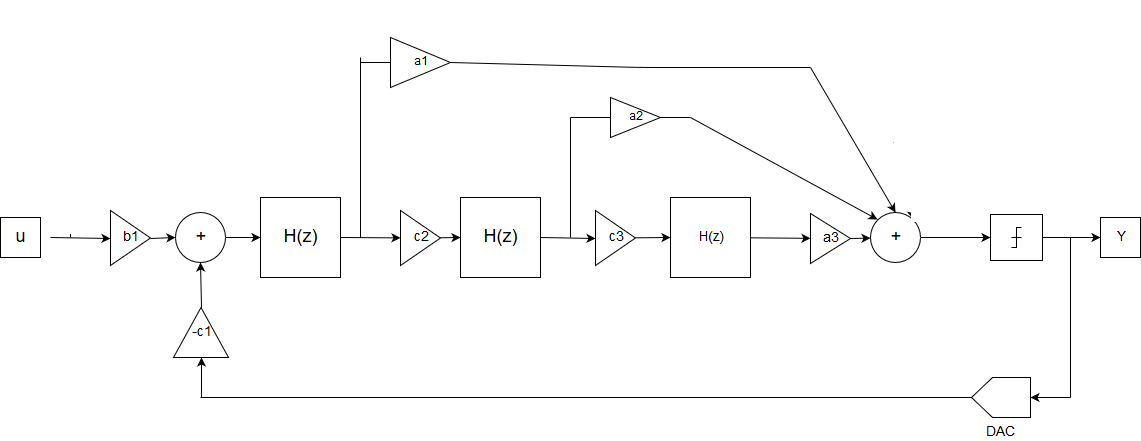
\includegraphics[width=\textwidth]{images/feedforward_no.png}
   \caption{Feedforward}
   \label{fig:forward}
\end{subfigure}

\caption{$3^{rd}$ order loop realization structures for feedforward and feedback}
\end{figure}

\subsection{Feedforward topology}
An example on the $3^{rd}$ order feedforward topology is depicted in figure \ref{fig:forward}. Unlike the feedback topology, this one has only one feedback from the quantized output. The coefficients ($a_1, a_2$ and $a_3$) are forwarded to the output, where their weight is added to the quantizer input. The STF and NTF are then given,

\begin{equation}
    STF = \frac{b_1(a_1H(z) + c_2a_2H^2(z) + c_2c_3a_3H^3(z))}{1 + b_1(a_1H(z) + c_2a_2H^2(z) + c_2c_3a_3H^3(z))}
\end{equation}

\begin{equation}
    NTF = \frac{1}{1 + b_1(a_1H(z) + c_2a_2H^2(z) + c_2c_3H^3(z))}
\end{equation}

By moving the coefficients to the summation node in front of quantizer, the signal presented at integrators output will be significantly lower than at the feedback topology. This leads to lesser swings and scaling, which means that the op-amp requirement can be relaxed, which leads to less power consumption. However one should be aware of operating on input amplitude near the reference voltage ($V_{ref}$), as this will drive the modulator to instability. The feedforward topology can further be improved by having a feedfoward path from input signal to the summation node in front of the quantizer, as shown in figure \ref{fig:input}. This means that the integrators do not process the input signal, only quantization noise $U$, and this leads to low distortion\cite[Ch.4.4.2]{Richard}, further relaxing the requirement for the integrator's op-amp. One thing to notice is that having fewer internal feedback DACs reduce the power dissipation significantly. 

\begin{figure}\label{final_top}
\centering
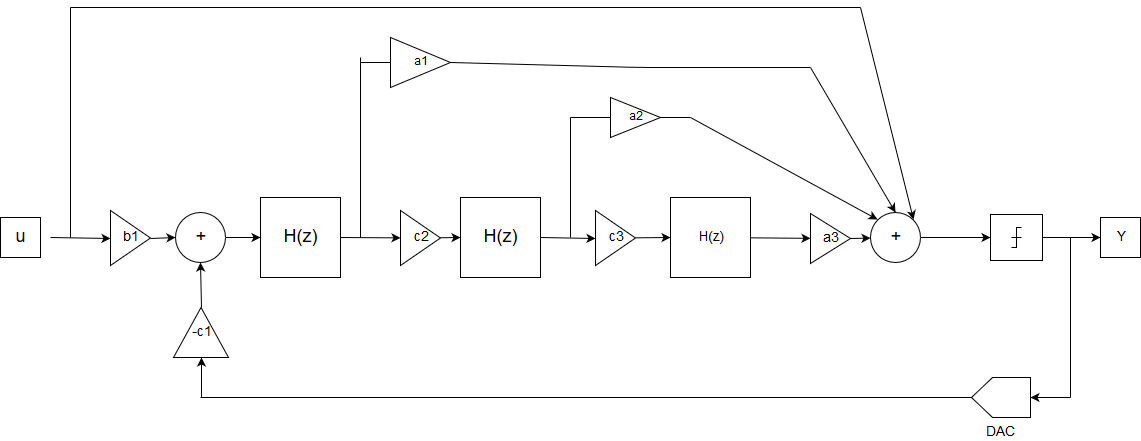
\includegraphics[scale=0.38]{images/feedforward.png}
\caption{$3^{rd}$ order feedforward topology with input signal forwarded to summation node}
\label{fig:input}
\end{figure}

\section{Time-domain}
The $\Delta\Sigma$ modulator can operate in a discrete-time domain (DT) or in the continuous-time domain(CT)\cite{Richard}. We have already seen how DT modulator operates in chapter 2. Figure \ref{fig:cont} illustrates a simple first order $\Delta\Sigma$ modulator. Unlike the DT $\Delta\Sigma$ modulator, the input signal and the integrator are continuous and the sampling occurs only before quantization. The STF and NTF for CT modulators has the same as the DT one.    

The main difference, is the way they are implemented. The DT $\Delta\Sigma$ modulators employ switched-capacitor (SC) integrators while CT systems use active-RC integrators in the modulators. To choose the right domain for a application, one has to look at the advantages and disadvantages of associated with each option.

Switched-capacitor has the perk of taking advantages on fine-line VLSI capabilities by eliminating the need to use physical resistors. Furthermore capacitors have high linearity, which is difficult to achieve with on-chip resistors in a standard CMOS process. In addition, the resistors in CT integrators can not afford to get too big as it can affect the thermal noise by increasing it, but having small resistors can increase the feedback capacitors, if one want to preserve the same settling time. 

The accuracy of SC integrators is good, since the transfer function of an SC circuit scales naturally with the clock frequency. The resistors and capacitors which get subjected to large production variation makes up the time-constants of CT integrators, which means that the accuracy of the CT integrators will be inferior to SC integrators\cite[Ch.6.6]{Richard}. Another advantage is that the SC systems is less sensitive to clock jitter.

The CT modulators is attractive to high-speed applications as it can achieve very high OSR, while SC modulators are limited by the achievable bandwidth of the opamps. Instead of having AAF outside the modulator as the DT modulator, the CT modulator has implicit AAF. The elimination of this filter can lead to power savings for the receiver.

\begin{figure}[H]
\centering
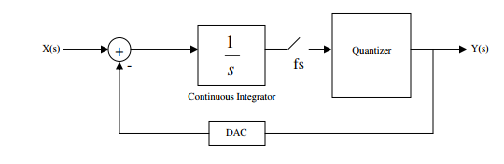
\includegraphics[scale=0.9]{images/cont.png}
\caption{Linear model of CT first order $\Delta\Sigma$ modulator}
\label{fig:cont}
\end{figure}

\section{Single-bit vs Multi-bit Quantizer}
For a full-scale, the quantization error is reduced by 6dB for every bit added to the resolution of the quantizer\cite[Ch.6]{Richard}. Meaning that the SQNR will increase with this amount leading to a more stable operation. This is especially good for modulators of high order. Also the feedback loop becomes more linear, consequently allowing us to choose NTF more aggressively. Hence even better SQNR can be obtained, and larger input signals can be used. This and more advantages makes multi-bit quantizer attractive to use. However the errors introduced by DACs is not attenuated as quantization errors. Since the DAC's output goes to the input signal, the errors will get injected with the signal. Consequently the linearity of the modulator is deepened on the  linearity of the DAC. Multi-bit quantizer struggles with being linear, and need costly corrections techniques to keep up with the high linearity demand. This is no problem for single-bit quantizer, since the DAC is inherently linear.

Another advantage with multi-bit quantizer is that it does not require large OSR as single-bit. Meaning the requirement for the bandwidth of a opamp can be relaxed. However adding more bits leads to a bigger power dissipation, making single-bit quantizer more attractive for applications that demand low power.

\section{Choosing architecture}
The requirement of the modulator is to achieve 16-bit resolution. Three things were considered in choosing the right architecture: area, power and requirement for the system. The final architecture that was selected was a discrete-time third-order single-bit single-loop feedforward architecture with input forwarded into the summation node, as shown in figure \ref{fig:input}.

The choice of modulator order was between second and third order, which both satisfied the specification with OSRs: 256 and 128 respectively. As the mentioned in section 3.1, the high OSR of second order can cause the quantization noise to become stronger. Furthermore, the high OSR also leads to stricter requirement for the opamp. The third order modulator takes bigger area and has stricter stability requirement, but having a relax requirement seemed more desirable. However the OSR was chosen to be 170, as we want the theoretical SQNR to be 10-20dB more than the desired SNR in order to allow degradation in SQNR due circuits non-idealities and leave as much of the noise budget for thermal noise\cite[Ch.9.2]{Richard}.

The feedforward topology was chosen because it gives the best $SNR_{peak}$. Moreover implementing feedback means that the power dispassion gets significantly larger, since the DAC's output is connected to the output of the integrators. One thing to remember is to have input amplitude a few dB under $V_{ref}$. Since $V_{ref}$ was chosen to be 1V, the input amplitude was chosen to be 0.5.

Finally, DT-time single-bit architecture is the most suitable for the application, since it is easier to implement an SC integrator, and it is the best option considering noise budget and power savings. Also, with the superior linearity that follows with single-bit architecture, makes it more desirable to implement considering the cost in power and complexity it will take to reach stability. The specifications for the modulator have been 
summarized in table \ref{spec}.

% Please add the following required packages to your document preamble:
% \usepackage{booktabs}
\begin{table}[H]
\centering
\caption{Specification for Modulator}
\label{spec}
\begin{tabular}{@{}ll@{}}
\toprule
Parameter       & Value        \\ \midrule
Resolution      & 16           \\
Fs              & 10MHz        \\
OSR             & 170          \\
Vdd             & 1.8V         \\
$V_{ref}$          & 1V           \\
Input amplitude & 0.5          \\
Order           & 3            \\
Topology        & Feed forward \\
Domain          & DT           \\
Quantizer level & 2            \\ \bottomrule
\end{tabular}
\end{table}